\documentclass[12pt,compress,aspectratio=169]{beamer}

\usetheme{metropolis}
\setbeamersize{text margin left=.5cm,text margin right=.5cm}
\setbeamertemplate{navigation symbols}{} % suppress nav bar
%\setbeamercovered{transparent}

\usepackage[utf8]{inputenc}
\usefonttheme{professionalfonts}
\usepackage{amsmath}
\usepackage{siunitx}
%\usepackage{graphicx}
\usepackage{tikz}
\usepackage{mathpazo}
%\usepackage[scaled]{helvet}
\usepackage{bm}
%\usepackage{xcolor,colortbl}
\usepackage{hyperref}

\sisetup{
  number-math-rm=\mathnormal,
  per-mode=symbol
}

\setmonofont{Ubuntu Mono}
\setlength{\parskip}{0pt}
\renewcommand{\baselinestretch}{1}


\title{Topic 1: Kinematics}
\subtitle{Advanced Placement Physics 1}
\author[TML]{Dr.\ Timothy Leung}
\institute{Olympiads School}
\date{June 29, 2020}

\newcommand{\iii}{\ensuremath\hat{\bm{\imath}}}
\newcommand{\jjj}{\ensuremath\hat{\bm{\jmath}}}
\newcommand{\kkk}{\ensuremath\hat{\bm{k}}}
\newcommand{\pic}[2]{\includegraphics[width=#1\textwidth]{#2}}
\newcommand{\mb}[1]{\ensuremath\mathbf{#1}}
\newcommand{\eq}[2]{\vspace{#1}{\Large\begin{displaymath}#2\end{displaymath}}}
\newcommand{\magdir}[2]{#1\text{ [#2]}}

\begin{document}

\begin{frame}{}

  {\LARGE
    \begin{center}
      \textbf{WELCOME TO AP PHYSICS}
    \end{center}
  }
\end{frame}



\begin{frame}{Pre-requisites}
  \begin{itemize}
  \item\textbf{Physics 11 and 12:} You will need to be comfortable with the
    topics covered in high-school level physics courses.
  \item\textbf{Vectors:} You need to be comfortable with vector operations,
    including addition and subtraction, multiplication/division by constants,
    as well as dot products and cross products.
  \end{itemize}
  If you already have a background in both differential and integral calculus,
  you may consider taking the AP Physics C exams instead.
\end{frame}



%\begin{frame}{AP Physics C Exams}
%  There are 2 AP Physics C exams, which are usually taken together on the same
%  day, in the first or second week of May of each year.
%  \begin{itemize}
%  \item Mechanics
%  \item Electricity and Magnetism
%  \end{itemize}
%  The Physics C exams are calculus based.
%\end{frame}



\begin{frame}{Classroom Rules}
  \begin{itemize}
  \item Treat each other with respect
  \item Raise your hands if you have a question. Don't wait too long
  \item E-mail me at \texttt{tleung@olympiadsmail.ca} for any questions related
    to physics and math and engineering
  \item Do \textbf{\emph{not}} try to find me on social media
  \end{itemize}
\end{frame}



\begin{frame}
  \titlepage
\end{frame}



\begin{frame}{Files for You to Download}
  \begin{itemize}
%  \item\texttt{PhysAPC-courseOutline.pdf}--The course outline
%  \item\texttt{PhysAPC-equationSheet.pdf}--Equation sheet for your exams
  \item\texttt{PhysAP1-01-kinematics.pdf}
  \item\texttt{PhysAPC-02-dynamics.pdf}
%  \item\texttt{PhysAPC-01-Homework.pdf}--Homework problems for Topic 1
%  \item\texttt{PhysAPC-02-Homework.pdf}--Homework problems for Topic 2
  \end{itemize}
  
  \vspace{.1in}Please download/print the PDF file for the class slides before
  each class. There is no point copying notes that are already on the slides.
  Instead, focus on things that aren't necessarily on the slides. If you wish
  to print the slides, we recommend printing \emph{four} slides per page.
\end{frame}



\begin{frame}{Vectors}
  Please refer to the handout to make sure that you are familiar with basic
  vector operations. We will be using a slightly more advanced notation method
  for this course.
\end{frame}



\section{Kinematics}

\begin{frame}{Kinematics}
  \textbf{Kinematics} is a discipline within mechanics concerning the
  motion of bodies. It describes the relationship between 
  \begin{itemize}
  \item<alert@1> Position
  \item<alert@1> Displacement
  \item Distance 
  \item<alert@1> Velocity
  \item Speed
  \item<alert@1> Acceleration
  \end{itemize}
  Kinematics does not deal with the causes of motion.
\end{frame}



\begin{frame}{Position}
  \textbf{Position} $\mb{x}$ describes the location of an object in a
  coordinate system. The origin of the coordinate system is called the
  ``reference point''. The SI unit for position is \textbf{meter}, \si{\metre}.
  
  \eq{-.2in}{
    \mb{x}(t)=x(t)\bm{\hat{\imath}} + y(t)\bm{\hat{\jmath}} + z(t)\bm{\hat{k}}
  }

  Vectors in 2D/3D Cartesian space are generally using the ``IJK notation''
  \begin{itemize}
  \item $\bm{\hat{\imath}}$, $\bm{\hat{\jmath}}$ and $\bm{\hat{k}}$ are
    \textbf{basis vectors} representing the directions of the $x$, $y$ and $z$
    axes. Basis vectors are \textbf{unit vectors} (i.e.\ length $1$)
  \item The IJK notation does not explicitly give the magnitude or the direction
    of the vector (needs to be calculated using the Pythagorean theorem)
  \end{itemize}
\end{frame}



\begin{frame}{Displacement}
  \textbf{Displacement} $\Delta\mb{x}(t)$ is the change in position from the
  initial position $\mb{x}_0$ within the same coordinate system. The unit for
  displacement is also meter.

  \eq{-.25in}{
      \Delta\mb{x}(t)=\mb{x}-\mb{x}_0
      =(x-x_0)\bm{\hat{\imath}}+
      (y-y_0)\bm{\hat{\jmath}}+
      (z-z_0)\bm{\hat{k}}
  }
  \begin{itemize}
  \item IJK notation makes vector addition and subtraction less prone to errors
  \item Since the reference point $\mb{x}_{\textrm{ref}}=\mb{0}$, the position
    vector $\mb{x}$ is also its displacement from the reference point
  \end{itemize}
\end{frame}



\begin{frame}{Distance}
  \textbf{Distance} $s(t)$ is a quantity that is \emph{related} to displacement.
  \begin{columns}
    \column{.7\textwidth}
    \begin{itemize}
    \item The length of the path taken by an object when it from $\mb{x}_0$ to
      $\mb{x}$
    \item A scalar quantity
    \item Always positive, i.e.\ $s\geq 0$
    \item Although the magnitude of the displacement vector is also a scalar,
      it is not necessarily the same as distance
    \item $s\geq |\Delta\mb{x}|$
    \end{itemize}
    
    \column{.3\textwidth}
    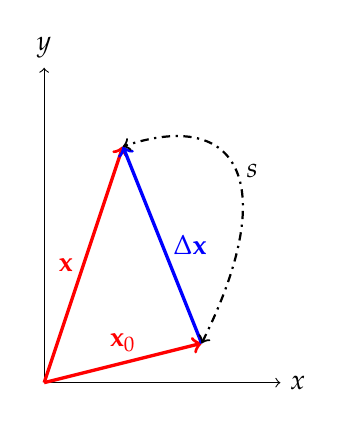
\begin{tikzpicture}[scale=.5]
      \draw[->](0,0)--(6,0) node[pos=1,right]{$x$};
      \draw[->](0,0)--(0,8) node[pos=1,above]{$y$};
      \draw[->,red,very thick] (0,0)--(4,1) node[midway,above]{$\mb{x}_0$};
      \draw[->,red,very thick] (0,0)--(2,6) node[midway,left]{$\mb{x}$};
      \draw[->,blue,very thick](4,1)--(2,6) node[midway,right]{$\Delta\mb{x}$};
      \draw[thick,dash dot,<->] (4,1)..controls (6,5) and (5,7)..(2,6)
      node[midway,right]{$s$};
    \end{tikzpicture}
  \end{columns}
\end{frame}




%
%
%
%\begin{frame}{Integrating Velocity to Get Position/Displacement}
%  Conversely, if $\mb{v}(t)$ is the time rate of change of position
%  $\mb{x}(t)$, then $\mb{x}$ is the time integral of $\mb{v}$:
%  
%  \eq{-.2in}{
%    \mb{x}(t)=\int\mb{v}(t)dt + \mb{x}_0
%  }
%  
%  The constant of integration $\mb{x}_0$ is the \emph{initial position} at
%  $t=0$. We can integrate each component to get $\mb{x}$:
%
% \eq{-.2in}{ \mb{x}(t)= \left(
%    \int v_x\bm{\hat{\imath}} +
%    \int v_y\bm{\hat{\jmath}} +
%    \int v_z\bm{\hat{k}}
%    \right) dt + \mb{x}_0
%  }
%\end{frame}



\begin{frame}{Average Velocity}
  \textbf{Average velocity} $\overline{\mb{v}}$ of an object is the finite
  displacement $\Delta\mb{x}$ over a \emph{finite} time interval $\Delta t$.
  The unit for velocity is \textbf{meters per second} (\si{\metre\per\second}):

  \eq{-.2in}{
    \boxed{
      \overline{\mb{v}}= \frac{\Delta\mb{x}}{\Delta t}
    }
  }
  
  Since the $\iii$, $\jjj$ and $\kkk$ directions ($x$, $y$, $z$ axes) are
  \emph{linearly independent} (what happens in one axis does not affect
  another), each component of average velocity can be calculated by separating
  each direction:

  \eq{-.15in}{
    \boxed{
      \overline{\mb{v}}=
      \frac{\Delta x}{\Delta t}\iii + \frac{\Delta y}{\Delta t}\jjj +
      \frac{\Delta z}{\Delta t}\kkk
    }
  }

  (Note: A bar is drawn over the symbol if it is averaged over time.)
\end{frame}



\begin{frame}{Instantaneous Velocity}

  \eq{0in}{
    \overline{\mb{v}}= \frac{\Delta\mb{x}}{\Delta t}
  }
  
  If displacement $\Delta\mb{x}$ is calculated a very small (in calculus, a very
  small change is called \emph{infinitesimal}) time interval $\Delta t$, then
  velocity is called the \textbf{instantaneous velocity}. 
\end{frame}



\begin{frame}{Instantaneous \& Average Speed}
  \textbf{Average speed} is similar to average velocity: it is the finite
  distance travelled over a finite time interval. Since distance is always
  positive, so too is the average speed
 
  \eq{-.2in}{
    \boxed{\overline{v}=\frac{s}{\Delta t}}
  }

  Likewise, when the time interval is made extremely small, then the speed is
  called the \textbf{instantaneous speed} $v$. Instantaneous speed $v$ is the
  magnitude of the instantaneous velocity vector.
\end{frame}



%\begin{frame}{Path}
%  Sometimes instead of explicitly describing the position $x=x(t)$ and $y=y(t)$,
%  the path of an object can be given in terms of $x$ coordinate $y=y(x)$, while
%  giving the $x$ (or $y$) coordinate as a function of time.
%  \begin{itemize}
%  \item In this case, substitute the expression for $x(t)$ into $y=y(x)$ to
%    get an expression of $y=y(t)$
%  \item Take derivative using chain rule to get $v_y=v_y(t)$
%  \end{itemize}
%\end{frame}


\begin{frame}{Instantaneous \& Average Acceleration}
  In the same way that velocity how quickly position changes with time, 
  \textbf{average acceleration} $\overline{\mb{a}}$ is the finite change in
  velocity $\Delta\mb{v}$ over a finite time interval $\Delta t$.
  The unit for acceleration is \si{\metre\per\second^2}.

  \eq{-.2in}{
    \boxed{
      \overline{\mb{a}} = \frac{\Delta\mb{v}}{\Delta t}
      =\frac{\mb{v}-\mb{v}_0}{\Delta t}
    }
  }
  
  Making the time interval $\Delta t$ infinitesimally small gives the
  \textbf{instantaneous acceleration} $\mb{a}(t)$.
%
%  \eq{-.2in}{
%    \mb{a}(t)= \frac{d\mb{v}(t)}{dt}=\frac{d^2\mb{x}(t)}{dt^2}
%  }
%
%
%
%  Acceleration is the second derivative of position, i.e.
%  \begin{enumerate}
%  \item Take derivative of $\mb{x}(t)$ to get $\mb{v}(t)=\mb{x}'(t)$
%  \item Take derivative again of $\mb{v}(t)$ to get $\mb{a}(t)=\mb{v}'(t)$
%  \end{enumerate}
\end{frame}



%\begin{frame}{Special Notation}{When Differentiating With Time}
%  Physicists and engineers often use a special notation when the derivative is
%  taken with respect to \emph{time}, by writing a dot above the variable:
%  \begin{itemize}
%  \item Velocity:
%
%    \eq{-.25in}{
%      \mb{v}(t)= \dot{\mb{x}}
%    }
%  \item Acceleration:
%
%    \eq{-.25in}{
%      \mb{a}(t)= \dot{\mb{v}}=\ddot{\mb{x}}
%    }
%  \end{itemize}
%  We will use this notation whenever it is convenient
%\end{frame}
%
%
%
%\begin{frame}{Integrating Acceleration to Get Velocity}
%  Velocity $\mb{v}(t)$ is the time integral of acceleration $\mb{a}(t)$:
%    
%  \eq{-.2in}{
%    \mb{v}(t)=\int\mb{a}(t)dt+\mb{v}_0
%  }
%
%  Again, we can integrate each component of the vector independently:
%
%  \eq{-.2in}{
%    \mb{v}(t)=
%    \left(\int a_x\bm{\hat{\imath}} +
%    \int a_y\bm{\hat{\jmath}} +
%    \int a_z\bm{\hat{k}}\right) dt +\mb{v}_0
%  }
%\end{frame}



\begin{frame}{If You Are Curious}
  For the curious minds (i.e.\ we don't need it for AP Physics), the change in
  acceleration in time is called \textbf{jerk}, with a unit of
  \si{\metre\per\second^3}:

  \eq{-.2in}{
    \overline{\mb{j}}= \frac{\Delta\mb{a}}{\Delta t}
  }

  The change in jerk in time is called \textbf{jounce} or \textbf{snap}, with a
  unit of \si{\metre\per\second^4}:
  
  \eq{-.2in}{
    \overline{\mb{s}}=\frac{\Delta\mb{j}}{\Delta t}
  }
  
  The next motion quantities are are called \textbf{crackle} and \textbf{pop},
  but these quantities are almost never used.
\end{frame}



\begin{frame}{Acceleration as Functions of Velocity and Position}
  Sometimes, acceleration are expressed as functions of velocity and position
  rather than of time, depending on the forces acting on them. For example:
  \begin{itemize}
  \item Gravitational or electrostatic forces: $a(x)=Ax^{-2}$
  \item Spring force: $\displaystyle a(x)=-Bx$
  \item Damping force (e.g.\ shock absorbers): $a(v)=Cv$
  \item Aerodynamic drag: $a(v)=Dv^2$
  \end{itemize}
  In these cases, solving for the motion quantities $x(t)$, $v(t)$ and $a(t)$
  requires calculus or numerical iterative methods.
\end{frame}



\section{Kinematic Equations}

\begin{frame}{Kinematic Equations}
  Without calculus, problems in AP Physics 1 only deal with
  \underline{constant acceleration}. Non-constant acceleration problems are
  studied in more depth in Physics C. The kinematic equations that will be used
  in Physics 1 are:
  \begin{columns}
    \column{.45\textwidth}

    \vspace{-.3in}{\Large
      \begin{align*}
        x &= x_0+ v_0t + \frac12at^2\\
        v &= v_0+at\\
        v^2 &= v_0^2+ 2a(x-x_0)
      \end{align*}
    }
    
    \column{.55\textwidth}
    \begin{itemize}
    \item Initial position: $x_0$
    \item Position at time $t$: $x$
    \item Initial velocity: $v_0$
    \item Velocity at time $t$: $v$
    \item Acceleration (constant): $a$
    \end{itemize}
  \end{columns}
  Kinematic equations are sometimes called the ``Big-five'' or ``Big-four''
  equations in Grade 11/12 Physics. In AP, you are given only three equations
  in your equation sheet.
\end{frame}



\section{Motion Graphs}

\begin{frame}{Motion Graphs}
  You should already be familiar with \emph{basic} motion graphs from Grade
  11/12 Physics:
  \begin{itemize}
  \item Position vs.\ time ($x$-$t$) graph
  \item Velocity vs.\ time ($v$-$t$) graph
  \item Acceleration vs.\ time ($a$-$t$) graph
  \end{itemize}
  Note that these graphs are only valid for 1D motion.
  %Depending on the situation, it may be more useful to plot motion
  %using other quantities as well.
\end{frame}



\begin{frame}{Uniform Motion}
  \textbf{Uniform motion} is when an object moves with constant velocity
  (neither magnitude nor direction changes) and therefore no acceleration. In
  1D, the motion graphs are:
  \begin{center}
    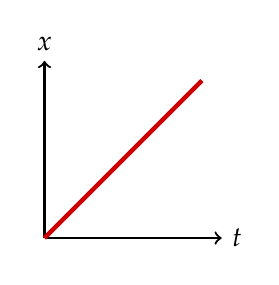
\begin{tikzpicture}[scale=.5]
      \draw[->,thick] (0,0)--(4.5,0) node[pos=1,right]{$t$};
      \draw[->,thick] (0,0)--(0,4.5) node[pos=1,above]{$x$};
      \draw[red!80!black,ultra thick](0,0)--(4,4);
    \end{tikzpicture}
    \hspace{.15in}
    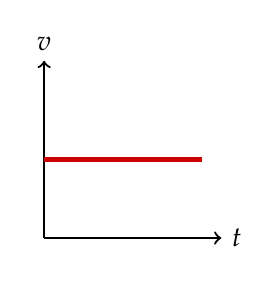
\begin{tikzpicture}[scale=.5]
      \draw[->,thick] (0,0)--(4.5,0) node[pos=1,right]{$t$};
      \draw[->,thick] (0,0)--(0,4.5) node[pos=1,above]{$v$};
      \draw[red!80!black,ultra thick](0,2)--(4,2);
    \end{tikzpicture}
    \hspace{.15in}
    \begin{tikzpicture}[scale=.5]
      \draw[->,thick] (0,0)--(4.5,0) node[pos=1,right]{$t$};
      \draw[->,thick] (0,0)--(0,4.5) node[pos=1,above]{$a$};
      \draw[red!80!black,ultra thick](0,0)--(4,0);
    \end{tikzpicture}
  \end{center}
  \begin{itemize}
  \item Constant velocity has a straight line in the $x$-$t$ graph
  \item The slope of the $x$-$t$ graph is the velocity $v$, which is constant
  \item The slope of the $v$-$t$ graph is the acceleration $a$, which is zero by
    definition
  \end{itemize}
\end{frame}



\begin{frame}{Uniform Acceleration}
  \textbf{Uniform acceleration} means that an object moves with a constant
  non-zero acceleration.
  \begin{center}
    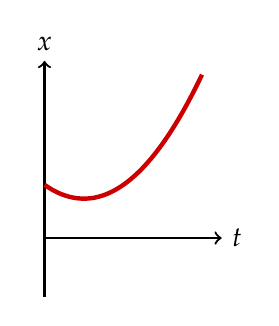
\begin{tikzpicture}[scale=.5]
      \draw[->,thick] (0,0)--(4.5,0) node[pos=1,right]{$t$};
      \draw[->,thick] (0,-1.5)--(0,4.5) node[pos=1,above]{$x$};
      \draw[smooth,samples=20,domain=0:4,red!80!black,ultra thick]
      plot({\x},{0.35*(\x-1)*(\x-1)+1});
    \end{tikzpicture}
    \hspace{.15in}
    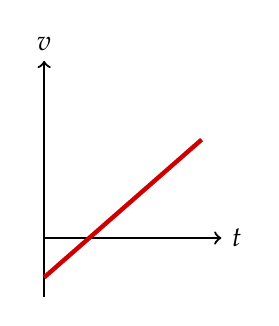
\begin{tikzpicture}[scale=.5]
      \draw[->,thick] (0,0)--(4.5,0) node[pos=1,right]{$t$};
      \draw[->,thick] (0,-1.5)--(0,4.5) node[pos=1,above]{$v$};
      \draw[red!80!black,ultra thick](0,-1)--(4,2.5);
    \end{tikzpicture}
    \hspace{.15in}
    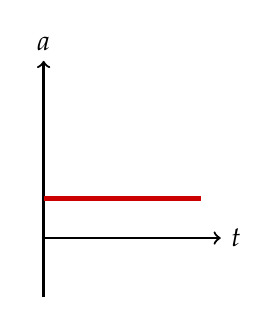
\begin{tikzpicture}[scale=.5]
      \draw[->,thick] (0,0)--(4.5,0) node[pos=1,right]{$t$};
      \draw[->,thick] (0,-1.5)--(0,4.5) node[pos=1,above]{$a$};
      \draw[red!80!black,ultra thick](0,1)--(4,1);
    \end{tikzpicture}
  \end{center}
  \begin{itemize}
  \item The $x$-$t$ graph is part of a \emph{parabola}
    \begin{itemize}
    \item If the parabola is \emph{convex} (opens up), acceleration is ($+$)
    \item If the parabola is \emph{concave} (opens down), acceleration is ($-$)
    \end{itemize}
  \item The $v$-$t$ graph is a straight line; its slope (a constant) is the
    acceleration
  \item The $a$-$t$ graph is a horizontal straight line
  \end{itemize}
\end{frame}



\begin{frame}{Simple Harmonic Motion}
  For \textbf{simple harmonic motions} (vibrations, oscillations), position,
  velocity and acceleration are non-constant, and they all change with time as
  sinusoidal functions.
  %Although we cannot use the kinematic equations here, we will be studying
  %this motion in the course.
  \begin{center}
    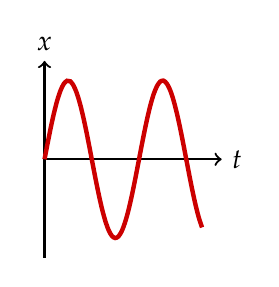
\begin{tikzpicture}[scale=.5]
      \draw[->,thick] (0,0)--(4.5,0) node[pos=1,right]{$t$};
      \draw[->,thick] (0,-2.5)--(0,2.5) node[pos=1,above]{$x$};
      \draw[smooth,samples=50,domain=0:4,red!80!black,ultra thick]
      plot({\x},{2*sin(150*\x)});
    \end{tikzpicture}
    \hspace{.15in}
    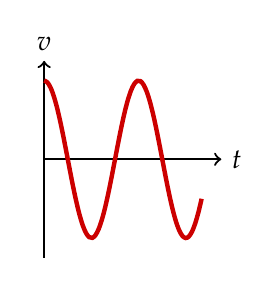
\begin{tikzpicture}[scale=.5]
      \draw[->,thick] (0,0)--(4.5,0) node[pos=1,right]{$t$};
      \draw[->,thick] (0,-2.5)--(0,2.5) node[pos=1,above]{$v$};
      \draw[smooth,samples=50,domain=0:4,red!80!black,ultra thick]
      plot({\x},{2*cos(150*\x)});
    \end{tikzpicture}
    \hspace{.15in}
    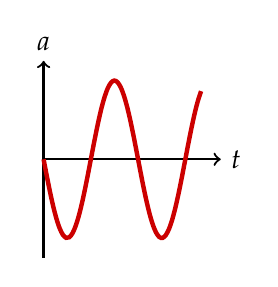
\begin{tikzpicture}[scale=.5]
      \draw[->,thick] (0,0)--(4.5,0) node[pos=1,right]{$t$};
      \draw[->,thick] (0,-2.5)--(0,2.5) node[pos=1,above]{$a$};
      \draw[smooth,samples=50,domain=0:4,red!80!black,ultra thick]
      plot({\x},{-2*sin(150*\x)});
    \end{tikzpicture}
  \end{center}
  \textbf{Bottom line}: regardless of the type motion,
  \begin{itemize}
  \item The $v$-$t$ graph is the slope of the $x$-$t$ graph
  \item The $a$-$t$ graph is the slope of the $v$-$t$ graph
  \end{itemize}
\end{frame}



\begin{frame}{Area Under Motion Graphs}
  \begin{columns}
    \column{.25\textwidth}
    \begin{center}
      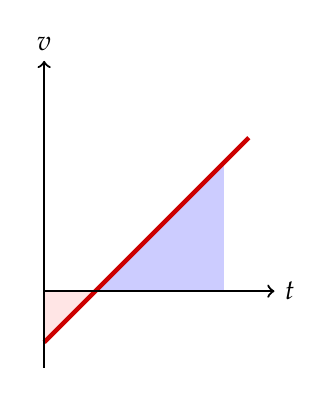
\begin{tikzpicture}[scale=.65]
        \draw[pink!40,fill=pink!40](0,0)--(0,-1)--(1,0)--cycle;
        \draw[blue!20,fill=blue!20](1,0)--(3.5,0)--(3.5,2.5)--cycle;
        \draw[red!80!black,ultra thick](0,-1)--(4,3);
        \draw[->,thick] (0,0)--(4.5,0) node[pos=1,right]{$t$};
        \draw[->,thick] (0,-1.5)--(0,4.5) node[pos=1,above]{$v$};
      \end{tikzpicture}
    \end{center}
    
    \column{.75\textwidth}
    The area under the $v$-$t$ graph is the displacement $\Delta x$:
    \begin{itemize}
    \item Area \textcolor{blue!20}{\emph{above}} the time axis: $+$
      displacement
    \item Area \textcolor{red!40}{\emph{below}} the time axis: $-$ displacement
    \end{itemize}
    \vspace{.1in}The area under the $a$-$t$ graph is the change in velocity
    $\Delta v$:
    \begin{itemize}
    \item Area \emph{above} the time axis: $+$ change in velocity
    \item Area \emph{below} the time axis: $-$ change in velocity
    \end{itemize}

    \vspace{.1in}The area under the $x$-$t$ graph has no physical meaning.
  \end{columns}
\end{frame}



\section{Projectile Motion}

\begin{frame}{Projectile Motion}
  A \textbf{projectile} is an object that is launched with an initial velocity
  of $\mb{v}_0$ along a parabolic trajectory and accelerates only due to
  gravity.
  \begin{center}
    \begin{tikzpicture}[scale=1.1]
      \draw[->](0,0)--(2,0) node[pos=1,right]{$x$};
      \draw[->](0,0)--(0,2) node[pos=1,above]{$y$};
      \draw[dotted,domain=0:6.25,thick] plot (\x, {1.2*\x-.2*\x*\x});
      \draw[ultra thick,->](0,0)--(.75,.9)node[pos=1,above]{$\mb{v}_0$};
      \draw[very thick,red!80!black,->]
      (0,0)--(0,.9)node[midway,left]{$v_{y1}$};
      \draw[very thick,blue!80!black,->]
      (0,0)--(.75,0)node[midway,below]{$v_x$};
      \draw[->](.5,0)arc(0:52:.5) node[pos=.6,right]{$\theta$};
    \end{tikzpicture}
  \end{center}
  \begin{itemize}
  \item $x$-axis usually is the \emph{horizontal} direction, with $+$ direction
    pointing \emph{forward}
  \item $y$-axis usually is the \emph{vertical} direction, with $+$ direction
    pointing \emph{up}
  \item The reference point is where the projectile is launched
  \item Consistent with the right-handed Cartesian coordinate system
  \end{itemize}
\end{frame}



\begin{frame}{Horizontal ($x$) Direction}
  The initial velocity $\mb{v}_0$ can be decomposed into its $x$ and $y$
  components using the launch angle $\theta$:

  \eq{-.2in}{
    \mb{v}_0=v_x\iii + v_{y0}\jjj =
    \left[v_0\cos\theta\right]\iii + \left[v_0\sin\theta\right]\jjj
  }

  There is no acceleration (i.e.\ $a_x=0$) in the horizontal direction,
  therefore $v_x$ is constant. The three kinematic equations reduce to a single
  equation:

  \eq{-.2in}{
    x=v_xt=\left[v_0\cos\theta\right] t
  }

  where $x$ is the horizontal position at time $t$ %, $v_0$ is the
  %magnitude of the initial velocity, $v_x=v_0\cos\theta$ is its horizontal
  %component.
\end{frame}




\begin{frame}{Vertical ($y$) Direction}
  There is constant acceleration due to gravity alone in the vertical
  direction, i.e.\ $a_y=-g$. (Acceleration is \emph{negative} due to the way we
  defined the coordinate system.) The important equation is this one:

  \eq{-.2in}{
    y = \left[v_0\sin\theta\right]t-\frac12gt^2
  }

  These two kinematic equations may also be useful:

  \vspace{-.2in}{\Large
    \begin{align*}
      v_y &= \left[v_0\sin\theta\right] -gt\\
      v_y^2&=\left[v_0^2\sin^2\theta\right]-2gy
    \end{align*}
  }
\end{frame}



\begin{frame}{Solving Projectile Motion Problems}
  Horizontal and vertical motions are independent of each other, but there are
  variables that are shared in both directions, namely:
  \begin{itemize}
  \item Time $t$
  \item Launch angle $\theta$ (above the horizontal)
  \item Initial speed $v_0$
  \end{itemize}
  
  \vspace{.2in}When solving any projectile motion problems
  \begin{itemize}
  \item \emph{Two} equations with \emph{two} unknowns
  \item If an object lands on an incline, there will be a third equation
    describing the relationship between $x$ and $y$
  \end{itemize}
\end{frame}



\begin{frame}{Symmetric Trajectory}
  A projectile's trajectory is symmetric if the object lands at the same height
  as when it launched.
  \begin{itemize}
  \item Time of flight
    \eq{-.1in}{t_\mathrm{max}=\frac{2v_0\sin\theta}{g}}
  \item Range
    \eq{-.1in}{R=\frac{v_0^2\sin(2\theta)}{g}}
  \item Maximum height
    \eq{-.1in}{y_\mathrm{max}=\frac{v_0^2\sin^2\theta}{2g}}
  \end{itemize}
  The angle $\theta$ is measured above the the horizontal.
\end{frame}



\begin{frame}{Maximum Range}
  \eq{-.1in}{R=\frac{v_0^2\sin(2\theta)}{g}}
  
  \begin{itemize}
  \item Maximum range occurs at $\theta=45^\circ$
  \item For a given initial speed $v_0$ and range $R$, launch angle $\theta$ is
    given by:
    
    \eq{-.2in}{
      \theta_1=\frac{1}{2}\sin^{-1}\left(\frac{Rg}{v_0^2}\right)
    }

    But there is another angle that \emph{gives the same range}!

    \eq{-.2in}{
      \theta_2=90^\circ-\theta_1
    }
  \end{itemize}
\end{frame}


\section{Relative Motion}

\begin{frame}{Relative Motion}
  \begin{columns}
    \column{.4\textwidth}
    \begin{tikzpicture}[scale=1.3]
      \draw[->](0,0)--(-.5,-.5)
      node[pos=1,left]{$x$}
      node[pos=0,above left]{$C$};
      \draw[->](0,0)--(1,0) node[pos=1,right]{$y$};
      \draw[->](0,0)--(0,1) node[pos=1,above]{$z$};

      \draw[->](2,3)--(1.5,2.5)
      node[pos=1,left]{$x'$}
      node[pos=0,above left]{$B$};
      \draw[->](2,3)--(3,3) node[pos=1,right]{$y'$};
      \draw[->](2,3)--(2,4) node[pos=1,above]{$z'$};

      \fill[red!70!black] (3,1) circle(.03) node[below right]{$A$};
      \draw[very thick,->,blue!70!black](0,0)--(2.98,.998)
      node[midway,below]{$\mb{x}_{AC}$};
      \draw[very thick,->,green!80!black](2,3)--(3,1.03)
      node[midway,right]{$\mb{x}_{AB}$};
    \end{tikzpicture}

    \column{.6\textwidth}
    \fbox{
      \begin{minipage}{.9\textwidth}
        All motion quantities must be measured relative to a frame of
        reference
      \end{minipage}
    }
    \begin{itemize}
    \item Two \textbf{frames of reference} (i.e.\ \textbf{coordinate systems})
      $C$ with axes $x,y,z$ and $B$ with axes $x',y',z'$
    \item The position of object $\textcolor{red!80!black}{A}$ can be described
      by $\textcolor{blue!70!black}{\mb{x}_{AC}}$ ($A$ relative to frame $C$) or
      $\textcolor{green!80!black}{\mb{x}_{AB}}$ ($A$ relative to frame $B$)
      \begin{itemize}
      \item It is clear that $\mb{x}_{AB}$ and $\mb{x}_{AC}$ are different
        because depending on which frame you measure from
      \item If the object moves, then $\mb{x}_{AB}$ and $\mb{x}_{AC}$ are
        functions of time
      \end{itemize}
    \end{itemize}
  \end{columns}
\end{frame}



\begin{frame}{Relative Motion}
  \begin{columns}
    \column{.4\textwidth}
    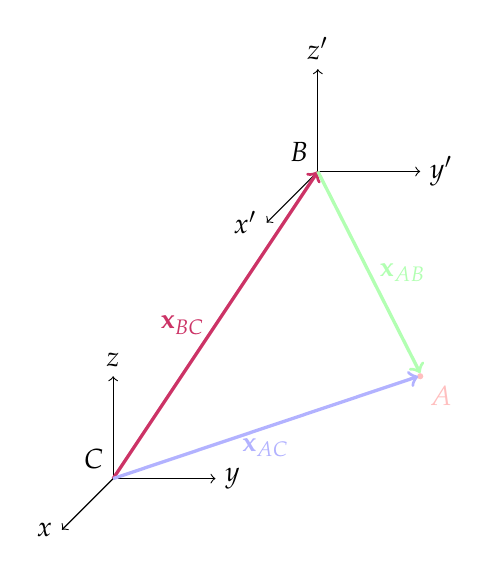
\begin{tikzpicture}[scale=1.3]
      \draw[->](0,0)--(-.5,-.5)
      node[pos=1,left]{$x$}
      node[pos=0,above left]{$C$};
      \draw[->](0,0)--(1,0) node[pos=1,right]{$y$};
      \draw[->](0,0)--(0,1) node[pos=1,above]{$z$};

      \draw[->](2,3)--(1.5,2.5)
      node[pos=1,left]{$x'$}
      node[pos=0,above left]{$B$};
      \draw[->](2,3)--(3,3) node[pos=1,right]{$y'$};
      \draw[->](2,3)--(2,4) node[pos=1,above]{$z'$};
      
      \draw[very thick,->,purple!80](0,0)--(2,3)
      node[midway,left]{$\mb{x}_{BC}$};
      \fill[pink] (3,1) circle(.03) node[below right]{$A$};
      \draw[very thick,->,blue!30](0,0)--(2.98,.998)
      node[midway,below]{$\mb{x}_{AC}$};
      \draw[very thick,->,green!30](2,3)--(3,1.03)
      node[midway,right]{$\mb{x}_{AB}$};
      
    \end{tikzpicture}

    \column{.6\textwidth}
    \begin{itemize}
    \item We can also relate the positions of the origins of the two frames of
      reference by $\mb{x}_{BC}$ (origin of frame $B$ relative to frame $C$)
      \begin{itemize}
      \item The vector pointing from the origin of frame $C$ to the origin of
        frame $B$
      \item If the two frames are moving relative to each other, then
        $\mb{x}_{BC}$ is a function of time
      \end{itemize}
    \item Without needing elaborate specific vector notations, it should be
      obvious that

      \eq{-.3in}{
        \textcolor{blue!70!black}{\mb{x}_{AC}}=
        \textcolor{green!80!black}{\mb{x}_{AB}}+
        \textcolor{purple!80}{\mb{x}_{BC}}
        }
    \end{itemize}
  \end{columns}
\end{frame}



\begin{frame}{Relative Motion}
  \begin{columns}
    \column{.4\textwidth}
    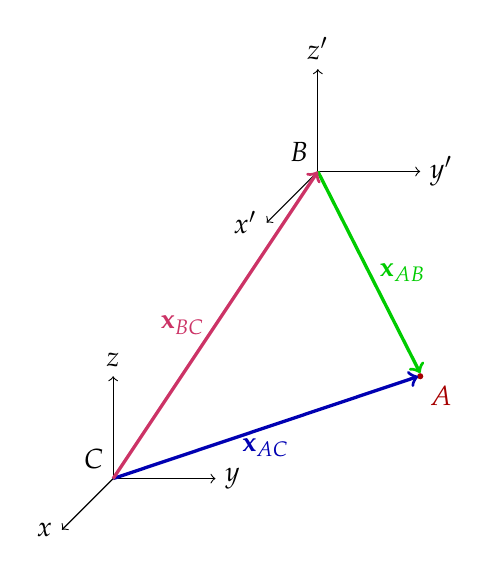
\begin{tikzpicture}[scale=1.3]
      \draw[->](0,0)--(-.5,-.5)
      node[pos=1,left]{$x$}
      node[pos=0,above left]{$C$};
      \draw[->](0,0)--(1,0) node[pos=1,right]{$y$};
      \draw[->](0,0)--(0,1) node[pos=1,above]{$z$};

      \draw[->](2,3)--(1.5,2.5)
      node[pos=1,left]{$x'$}
      node[pos=0,above left]{$B$};
      \draw[->](2,3)--(3,3) node[pos=1,right]{$y'$};
      \draw[->](2,3)--(2,4) node[pos=1,above]{$z'$};

      \fill[red!65!black] (3,1) circle(.03) node[below right]{$A$};
      \draw[very thick,->,blue!70!black](0,0)--(2.98,.998)
      node[midway,below]{$\mb{x}_{AC}$};
      \draw[very thick,->,green!80!black](2,3)--(3,1.03)
      node[midway,right]{$\mb{x}_{AB}$};
      \draw[very thick,->,purple!80](0,0)--(2,3)
      node[midway,left]{$\mb{x}_{BC}$};
    \end{tikzpicture}

    \column{.6\textwidth}
    Starting from the definition of \textbf{relative position}:

    \eq{-.2in}{
      \textcolor{blue!70!black}{\mb{x}_{AC}}=
      \textcolor{green!80!black}{\mb{x}_{AB}}+
      \textcolor{purple!80}{\mb{x}_{BC}}
    }
    
    \vspace{-.15in}Using the definitions for velocity to get a similar
    equation for \textbf{relative velocity}:

    \eq{-.2in}{
      \textcolor{blue!70!black}{\mb{v}_{AC}} =
      \textcolor{green!80!black}{\mb{v}_{AB}}+
      \textcolor{purple!80}{\mb{v}_{BC}}
    }

    \vspace{-.15in}Likewise, \textbf{relative acceleration} has a similar
    expression:

    \eq{-.3in}{
      \textcolor{blue!70!black}{\mb{a}_{AC}}=
      \textcolor{green!80!black}{\mb{a}_{AB}}+
      \textcolor{purple!80}{\mb{a}_{BC}}
    }
  \end{columns}
\end{frame}



\begin{frame}{Relative Velocity Example}
  If an airplane ($P$) flies in windy air ($A$) we must consider the velocity
  of the airplane relative to air, i.e.\ $\mb{v}_{PA}$ and the velocity of the
  air relative to Earth $E$, i.e.\ $\mb{v}_{AE}$. The velocity of the airplane
  relative to Earth is therefore

  \eq{-.2in}{
    \mb{v}_{PE}=\mb{v}_{PA}+\mb{v}_{AE}
  }

  \textbf{Simple example:} If an airplane is flying at a constant velocity of
  \SI{253}{km/h} south relative to the air and the air velocity is
  \SI{24}{km/h} east, what is the velocity of the airplane relative to Earth?
\end{frame}



\begin{frame}{Relative Velocity}
  In classical mechanics, the equation for relative motion follows the
  \textbf{Galilean velocity addition rule}:

  \eq{-.25in}{
    \mb{v}_{AC}=\mb{v}_{AB}+\mb{v}_{BC}
  }

  \vspace{-.1in}The velocity of $A$ relative to reference frame $C$ is the
  velocity of $A$ relative to reference frame $B$, plus the velocity of $B$
  relative to $C$. If we add another reference frame $D$, the equation becomes:

  \eq{-.25in}{
    \mb{v}_{AD}=\mb{v}_{AB}+\mb{v}_{BC}+\mb{v}_{CD}
  }
\end{frame}


\begin{frame}{Typical Problems}
  In the AP Physics 1 exam, questions involving kinematics usually appear in the
  multiple-choice section. The problems themselves are not necessarily very
  different from Grade 11/12 Physics problems, but:
  \begin{itemize}
  \item You have to solve problems faster because of time constraint
  \item You can use $g=\SI{10}{m/s^2}$ in your calculations to make your lives
    simpler
  \item A lot of problems are \emph{symbolic}, which means that they deal with
    the algebraic expressions, not actual numbers
  \item Will be coupled with other types (e.g.\ dynamics and rotational) in
    the free-response section
  \item You \emph{will} be given an equation sheet
  \end{itemize}
\end{frame}


\end{document}
